\documentclass[12pt, oneside, letterpaper]{report}
%\usepackage{ifpdf}
%\usepackage[colorlinks,bookmarksopen]{hyperref}
\usepackage{layout}
%\usepackage{lscape}
\usepackage{verbatim}
\usepackage{graphicx}
\usepackage{listings} %for source code figures
\textwidth=475pt
\hoffset=-.5in
\begin{document}
% ----------------------------------------------- front matter of the document
%\maketitle
\part{System and Software Design Description (SSDD): Incorporating
     Architectural Views and Detailed Design Criteria \\ for \\ Hatch}
\tableofcontents                                % chapter with the table of contents
\listoffigures
\listoftables
%------------------------------------------------ body of the document
\chapter{Introduction}

%%%%%%%%% SUMMARY -- 1 page, third person
% e.g:  "The PI will prove" not "I will prove"

%Introduction / Summary (1 page).  The following information is typically included in proposal introductions for this 
%grant. The summary should lead to the proposal body but it should also be a self-contained document, 
%summarizing what is being proposed and why.   
 
% Provide appropriate background that sets the context for the problem and the objectives. 
%State the specific problem (may also be thought of as a need, central research question, or hypothesis) 
%your research will address. 
% State the objectives of the proposed research. 
%State any limits of the proposed research  (may not be needed). 
%Summarize the research methods you will use to achieve research objectives (if clearly covered elsewhere 
%in the introduction, a separate section may not be needed). 


%\required{Project Summary}
\section{Project Summary}
% This should be a brief statement of the problem you plan to address.
% It should look something like an abstract. 
In today's scientific environment, there is a growing focus on data storage and
processing. Some of the largest problems scientists face are related to the data
deluge, and the inability to conceptalize problem and solutions from large
tracts of data. The result is many attempts by scientific professionals to 
design software, leading to many bad software designs. Vast amounts of 
expensively collected data never get processed, 
because the software designs take so much maintenance. Data is often duplicated,
often in different locations, lost, or never makes it from collection to 
analysis. The overall lack of system designs to handle the data further 
hinders analysis.

This proposal is for a project that helps solve these design problems for 
many scientists. The project is a data harvester and organizer tool. It
is a local web interface that allows scientists to collect, query, organize, 
and share data with other researchers.
Many of these scientists work with similar data sets, ask different 
questions, and need immediate search tools. The proposed tool would first allow 
users to visualize and filter data, and secondly prepare and ship the data
off for analysis. It also helps users visualize data graphically, to 
help the conceptualize, organize, and refine data, before transporting and 
processing it. This 
project proposes using PTAG and othe ecological data sets from the Columbia 
Basin to test design, but should be exdendable to many different users with very
different data sets.

The tool will not overlap with the functionality of existing tools like 
PTAGIS or DART. It will carefully handle data sharing,
choosing opt-in, lock-down policies by default.

\subsection{Background}
%this section needs more stats and citations
In the Columbia Basin today, millions of federal dollars are spent on PTAG 
and othe systems to collect environmental data. 
This data includes fish location, ecological community composition, and 
abiotic data. Yet, the project 
results from most research are far from concrete. Despite the lack of 
understandable results, important decisions that affect the local environment 
and economy have to be made. Decisions like whether or not to conduct 
major habitat restoration projects. 

%We should cite something other study / examples in the basin. Foster's talk
% just sticks in my head as a good example
The Columbia Basin is just one small example. Bioinformatics is another 
data intesive study that generates more data that it can process. Its 
%is this 10%? It may be lower
estimated that less than 10\% of the data collected by bioinformatic 
researchers at the University of Idaho actually makes it through proccessing
\cite{foster}. The rest has to be filtered as best as can be managed, and the 
low value data trimmed out. The problem with 10\% data use, is that not just 
the fat, but the meat and bone has to be cut away. Either significantly more
data must be analyzed, or significantly less should be collected. At the very
least, storing the data in an easily readable format can show where the 
gaps are. So far, our experience and research shows similar shortfalls in 
data analysis in the Columbia Basin.

\subsection{Problem Statement}
One of the biggest problems researchers in the Columbia Basin have is getting
their data somewhere meaningful. Central databases like PTAGIS offer a 
central storage and clients can push data there, but they don't offer useful
tools for managing data. Once the data is pushed, it is hard to access and
manipulate. 
%stuff to massage
% I hate to get rid of the next bit, because it is some of the buzz that the
% project approvers are looking for. Can we work this verbage in without it
% being a priority / main focus?
Researchers are often in remote locations, and have low bandwidth
connections. 
% end stuff to massage
Creating a robust tool will guarantee ease of use for the data, no matter
the location.

Many researchers have significant data management tasks before even thinking 
about pushing data to the cloud. Once they are ready, they need seemless ways to
synchronize data to and from the cloud. They also may want to query their data,
and filter it into small subsets. Most researchers don't have time to learn
new programming language or interfaces. They need a data management tool 
that has a user 
interface that is familiar to use cases they already understand. Once they
have created a data subset, they will want to share it, save it, copy it, 
and compare it with other data sets. Getting the right data to the right place 
in the right amount of time is crucial.

\subsection{Objectives}

\begin{figure}[!h]
        \begin{center}
		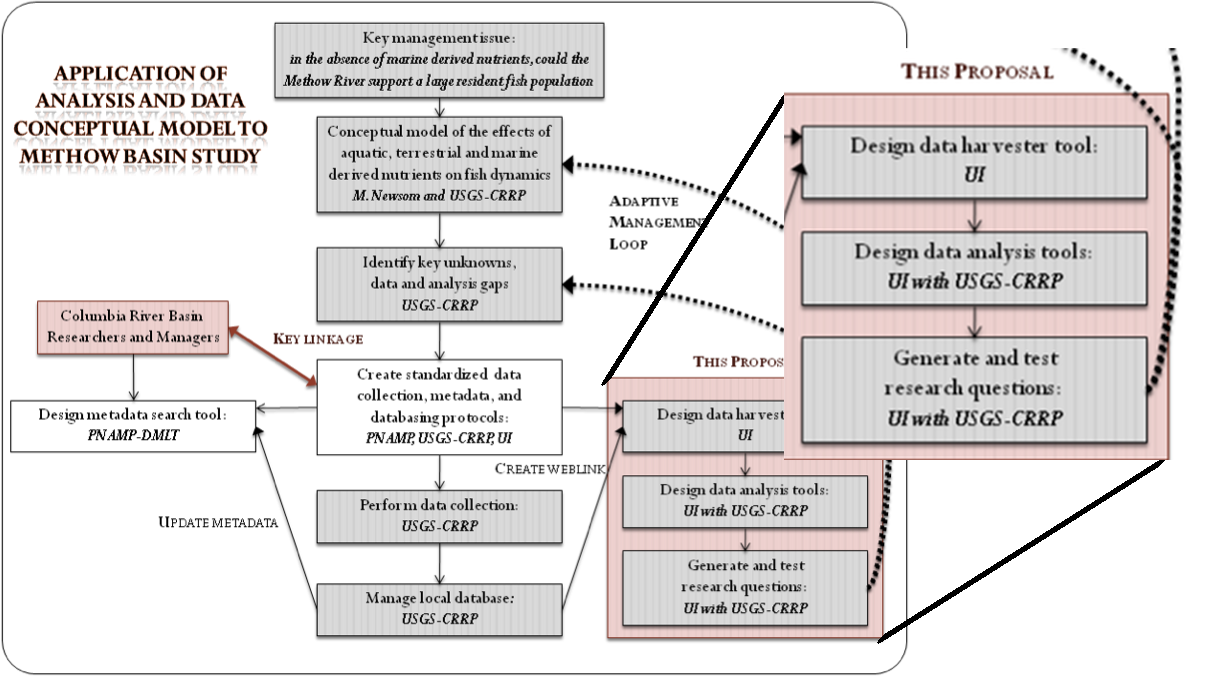
\includegraphics[width=120mm]{images/combo_proposal}
                \caption{This proposal software's application domain in DE-CRRP}
                \label{combo_proposal}
        \end{center}
\end{figure}

The proposed project will tackle the UI data harvester portion of the grant 
funded USGS-CRRP project (Figure \ref{combo_proposal}), directed by Alex 
Fremier of the UI College of Natural Resources. The data management tool
will be a web-like GUI that can be installed locally on the clients' computers.
The tool will contain a expandable meta data server 
that can be connected to others, for a \textbf{decentralized} data storage
cloud. The cloud will consist of the many instances of the tool, acting as a
cloud of 
\textbf{decentralized databases}. It will contain an interface to an existing 
or custom \textbf{networking protocol} that will allow for many different data 
formats to be synchronized across the cloud. The project will also have graphic
interfaces for \textbf{seamless data management}.

The decentralized cloud model allows some serious advantages to researchers.
They can see exactly what their data looks like, before they submit it.
They can filter out bad data before it consumes bandwidth, and can retract
undesirable data from the cloud, even after synchronizing it. It also frees
them from central storage service management and fees, and 
\textbf{encourages internode and inter-research communication}. 
The tool can be setup
on multiple hosts, and can be used for the benefits of 
the centralized cloud model. Each client can decide what topology suites them 
best.

The decentralized cloud model implements a distributed database model.
Distributed databases increase availability and reliability. They are more
easily expandable, and can better protect from data loss from local disasters or
malicious attacks. Moving data to where it is in highest demand also increases
query performance. Offloading archive data to remote site with more 
resources preserves local resources. Replicated datasets can guarantee 
better availability. By staging data locally and filtering it before allowing
it to be exchanged, the autonomy of the organization is better preserved. 

%probably some specific network protocols, like SOAP, etc, should be mentioned
%Alex, the network protocol doesn't have to apply just to low bandwidth users
%, but also to large data transfers
The network protocol will allow incremental synchronization of data from host
to host, even in less reliable environments. The tool will create
an \textbf{outreach} from researchers in high availability areas to those
in low availability, low bandwidth areas, and back. The network protocol
will have support for major data formats (i.e. SQL, CSV, more), and allow
users to send incremental pieces of the data. In the case of very large 
data sets or low bandwidth, the receiver of the data can still use it. Whether 
the data takes more time to transfer, or never completes.

The seamless interface will allow users to sort their data needing only 
basic knowledge of computers. Users will be able their mouse to select
datasets and apply filters to them. The tool will allow them to query local or
remote data, or to dynamically join both. Queries will create data subsets that
users can bring to a workspace. The tool will be able to sort data however
the user likes, on the fly. It will then be able to graph the ranges in 
the subset in most ways the user could want to sort them.

Once the user has manipulated their data subset to their satisfaction, they
will be able to save it in the meta data server's format, or in a set of major
data formats. The tool will also have analysis modules that will allow them
to run analysis on the local host. These modules will be extensible to running 
analysis jobs on other designated compute hosts, like workstations, clusters,
or even Amazon's EC2. The tool will come only with basic functionality for 
local analysis modules, but will be extensible to the heavier compute options.
%\required{Intellectual Merit}
% This is why your project is interesting and will help further
% knowledge in the field of mathematics. 

%\required{Broader Impacts}
% There are 4 kinds of broader impacts.
% 1. advance discovery and understanding while promoting teaching,
% training and learning
% 2. broaden the participation of underrepresented groups
% 3. disseminated broadly to enhance scientific and technological
% understanding
% 4. benefits of the proposed activity to society




%------------------------------------------------
\begin{comment}

	\section{Identification}
		The software system being considered for development is referred
		to as Groups in a University Setting or gus. The customer providing
		specifications for the ethnic and religion team is the Lutheran
		Campus Ministry. The ultimate customer, or end-user, of the system
		will be student groups at the University of Idaho. This is a new
		project effort, so the version under development is version 0.05
	\section{Purpose}
		The purpose of the system under development is to provide a tool
		for the easy administration and tracking of university-style groups
		including but not limited to clubs and sports teams, the system will
		also try to increase student involvement by connecting and recognizing
		the involvement of users. While the system will be used by university
		personnel, this document is intended to be read and understood by UICS
		software designers and coders.  This document will also be approved by
		Dr. Clinton Jeffery.
	\section{Scope}
		GUS is to social-networking as an intranet is to the Internet.
		Where other social networks distract users with non-university
		non-local non-face-to-face non-involvement, GUS will focus these
		types of functionalities to the university and local community
		setting to best meet the administrative and service needs of groups
		in a university setting.  In addition to being a group-centered
		student-involvement web-application.
	\section{Definitions, Acronyms, and Abbreviations}
		\begin{tabular}{|p{4cm}|p{10cm}|}
		\hline
		\textbf{Term or Acronym} & \textbf{Definition} \\ \hline
		Alpha test & Limited release(s) to selected, outside testers \\ \hline
		Beta test & Limited release(s) to cooperating customers wanting early access to developing systems \\ \hline
		Final test & aka, Acceptance test, release of full functionality to customer for approval \\ \hline
		DFD & Data Flow Diagram \\ \hline
		SDD & Software Design Document, aka SDS, Software Design Specification \\ \hline
		SRS &  Software Requirements Specification \\ \hline
		SSRS & System and Software Requirements Specification \\ \hline
		GUS & Groups in a University Setting \\ \hline
		\end{tabular}
	\section{References}
		\begin{enumerate}
	\item www.churchteams.com
	\item www.groupmeister.com
	\item www.teamr.com
	\item www.salesboom.com
	\item www.wikipedia.org
\end{enumerate}
	\section{Overview and Restrictions}
			This document is for limited release only to UI CS personnel
	working on the project.

		Section 2 of this document describes the system under development
		from a holistic point of view.  Functions, characteristics,
		constraints, assumptions, dependencies, and overall requirements
		are defined from the system-level perspective.

		Section 3 of this document describes the specific requirements of
		the system being developed.  Interfaces, features, and specific
		requirements are enumerated and described to a degree sufficient
		for a knowledgeable designer or coder to begin crafting an
		architectural solution to the proposed system.

		Section 4 provides the requirements traceability information for
		the project.  Each feature of the system is indexed by the SSRS
		requirement number and linked to its SDD and test references.

		Sections 5 and up are appendices including original information
		and communications used to create this document.

\nopagebreak
\chapter{Constraints and Stakeholder Concerns}

	\section{Constraints}
				\subsection{Environmental Constraints}
		\subsection{System Requirement Constraints}
		\subsection{User Characteristic Constraints}
	%\section{Stakeholder Concerns}
	%	\include{SSRS/StakeholderConcerns.tex}

%\chapter{System and Software Architechture}
%			\section{Users Architectural View}
		\subsection{User's View Identification}
		\subsection{User's View Representation and Description}
	\section{Developer's Architectural View}
		 \subsection{Developer's View Identification}
		 \subsection{Developer's View Representation and Description}
			\subsubsection{Object Model}
			\subsubsection{Dynamic Model}
		 \subsection{Developer's Architectural Rationale}
	\section{Consistency of Architecutural Views}
		\subsection{Developer's Viewpoint Detailed Software Design}
		\subsection{Component Dictionary}
		\subsection{Component Detailed Design}
			\subsubsection{Detailed Design for Component/Entity: Name of Component}
			\subsubsection{Detailed Design for Component/Entity: Name of Component}
			\subsubsection{Detailed Design for Component/Entity: Name of Component}
			\subsubsection{Detailed Design for Component/Entity: Name of Component}
	\section{Data Dictionary}

%------------------------------------------------
\end{comment}

\chapter{Requirements Traceability}
		\section{Customer Requirements}
			\section{Database}

\subsection{Introduction}
One of the biggest challenges with Hatch was how to organize data. Specifically, pretty
much every organization with scientific data has their own standard or format on 
how they store research data. Many of these organizations want to share data between 
each other, but they cannot decide how to merge the formats. Consider the following
examples:

\begin{figure}[h]
	\begin{center}
	\begin{tabular}{ | c | c | c | }
		\hline
		site	&	datetime		&	unique fish tag	\\
		\hline
		TUC	&	02/16/06 19:08:15 	&	3D9.1BF1E7919A 	\\
		TUC	&	02/16/06 19:18:36 	&	3D9.1BF1A998FA 	\\
		TUC	&	02/17/06 18:21:03 	&	3D9.1BF20E8FE2	\\
		...	&	...			&	...		\\
		\hline
	\end{tabular}
	\caption{A database representing for PTAGIS data} 
	\label{ptagis_ex1}
	\end{center}
\end{figure}

\begin{figure}[h]
	\begin{center}
	\begin{tabular}{ | c | c | }
		\hline
		unique fish tag	&	DNA sequence	\\
		\hline
		3D9.1BF1E7919A 	&	ATGCTTAC...	\\
		3D9.1BF1A998FA 	&	TTACGATC...	\\
		3D9.1BF20E8FE2	&	GTGGASCT...	\\
		...		&	...		\\
		\hline
	\end{tabular}
	\caption{A database representation for DNA data} 
	\label{dna_ex1}
	\end{center}
\end{figure}

In each of the examples above, the data is represented with \textbf{rows} and 
\textbf{columns}, much the same way someone would represent the data in a Microsoft
Excel spreadsheet. These structures in a typical \textbf{relational database} (SQL, etc).
are called \textbf{tables}.

The above examples are simplifications of the rows and columns in actual research 
data. But they highlight one of the biggest issues with data storage using relational
databases: they require you to know the column names ahead of time. Not only that,
but they require that you know the data types of the values that go in those columns,
and once a table is created expecting a certain format, it is hard to change.

The problem with needing to know the structure of research data before designing
databases, is that research data \textbf{is semi-structured}, at best. Once it does
represent some structure, it often changes. For example, once researchers finally 
decide what columns and data types should go in the table in Figure \ref{ptagis_ex1},
another researcher suggests more columns that should go in to the table.

This leads to endless edits to the database and program design by some software 
developer. The standard table format that everyone can agree on isn't useful to many
researchers, because it usually leaves out a lot of other needed columns and fields.

A better approach is needed. Researchers, not committees, should decide how to store 
data. Data should be mergable based on common values in different tables (like the 
\textbf{unique fish tag} column in Figures \ref{ptagis_ex1} and \ref{dna_ex1}. The 
person who inputs the data should decide how one particular dataset is stored in a 
database, and should be able to choose to store the same data in a different table 
format, how they choose. There should be a simple tool that helps them do this.

The following sections describe different approaches to implementing a database design
that enables data storage for dynamic or semi-structured data.


\subsection{Relation Databases with table creations}
This approach is the simplest and follows the concept of table creation for data sets
pretty closely. Basically, for each input document in the form of a spreadsheet, a new
SQL table is created. The columns names and type are determined from the headers and 
data values in the spreadsheet.

\begin{figure}[h]
	\begin{center}
	\begin{lstlisting}
		CREATE TABLE ptagis_doc1
			(
				id int, 
				site char(50), 
				read_data_time date,
				tag char(50)
			); 
	\end{lstlisting}
	\caption{The SQL syntax for creating the table in Figure \ref{ptagis_ex1} } 
	\label{ptagis_ex1_sql}
	\end{center}
\end{figure}

The biggest problem with this approach with this approach is that each document
in the database is a table. When searching for a specific document, the database 
typically searches for the table name. This search is linear, and with hundreds,
thousands, or hundreds of thousands of documents, frequently searching the database
to look for values would be infinitely slow and useless.

Another problem with this design, is that building an interface like a web gui would
be difficult and complicated. 


\subsection{Relational Databases with tables for each datatype}
Another approach is to create column tables for each data type, and let document 
tables just be collections of columns. Each of the document column values point to 
respective values in the column tables.

\begin{figure}[h]
	\begin{center}
	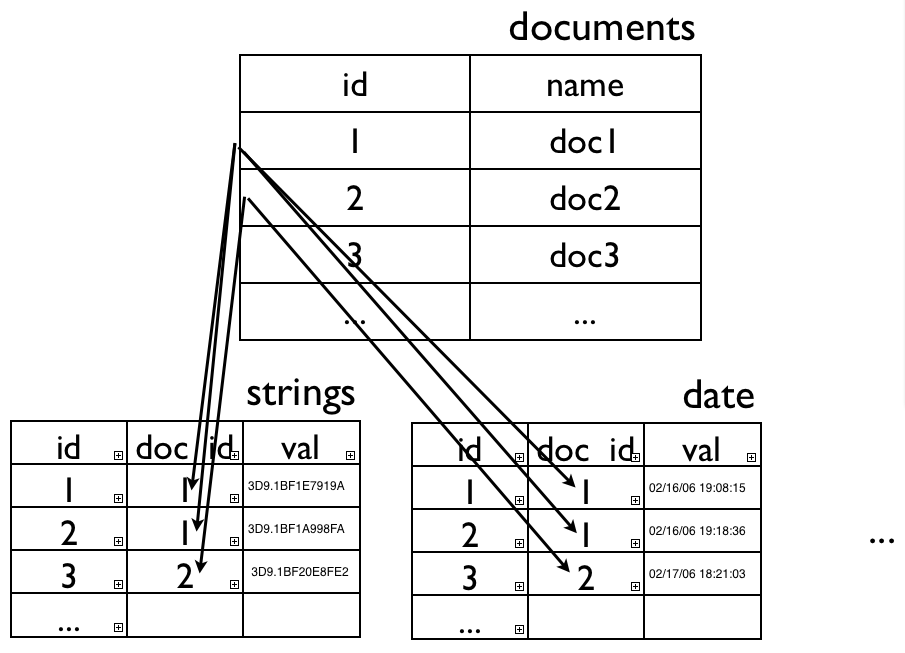
\includegraphics[width=80mm]{images/rel_db_lookup}
	\caption{Document table as a lookup table} 
	\label{rel_db_lookup}
	\end{center}
\end{figure}

This allows for documents to have a dynamic amount of columns with variable data types.
But there are two problems with this approach. First, for every value in every document
in the database, they are put into one table (i.e. all values with a 'string' data type
go into the 'string' table). With potentially millions of data values, each table
becomes an overflowing bucket, and don't utilize the the advantages of storing multiple
columns and values in one table. Searches for data would require lots of filtering 
for just the ones wanted for specific doucments, and would be inefficient.

The other issue is that every retrieval of data from a document would require lot and 
lots of lookups. Data retrieval over significantly high data sets would quickly become
very computationally intensive, and not practical.


\subsection{CouchDB}
When one thinks about the fundemental issues with storing, searching, and merging 
research data, a core issue is identified: data is semi-structured. This is what
makes trying to use relational databases so hard. They were made for datasets where
you knew the structure up front, and seldom wanted to change their structures.

The one assumption that Hatch makes about the data is that \textbf{there are rows and
columns}. This is the only assumption Hatch makes. This leaves the database and 
interface designs free from whatever changes are needed by the users.

This is done by storing data in JSON format. The data is stored in an array of hashes,
modeled exactly like how Ruby on Rails 3 returns records from its Active Record.
This allows users to input data however they like, define delimiters for columns using
Hatch Input Filters, and Hatch does the rest. It finds the most specific data type the
values can be stored in, skips non-matching entries, and populates all the forms on 
the web pages according to the data. All without actually knowing the structure of the 
data.

This leads to the technical implementation of the Hatch Database.


\subsection{Hatch Database}
Since Hatch uses Ruby on Rails, there are lots of tools and libraries for using the 
standard relational database, via Rails' Active Record. In many/most cases, Hatch
actually wants to stick to the relational database. With Hatch's internal database
structured, order is important. For example, a user will always have a name, email
address, etc. A document will always have a name and an owner. But the data in the
document is the semi-structured data. Hatch only wants to use CouchDB for that.

\begin{figure}[h]
	\begin{center}
	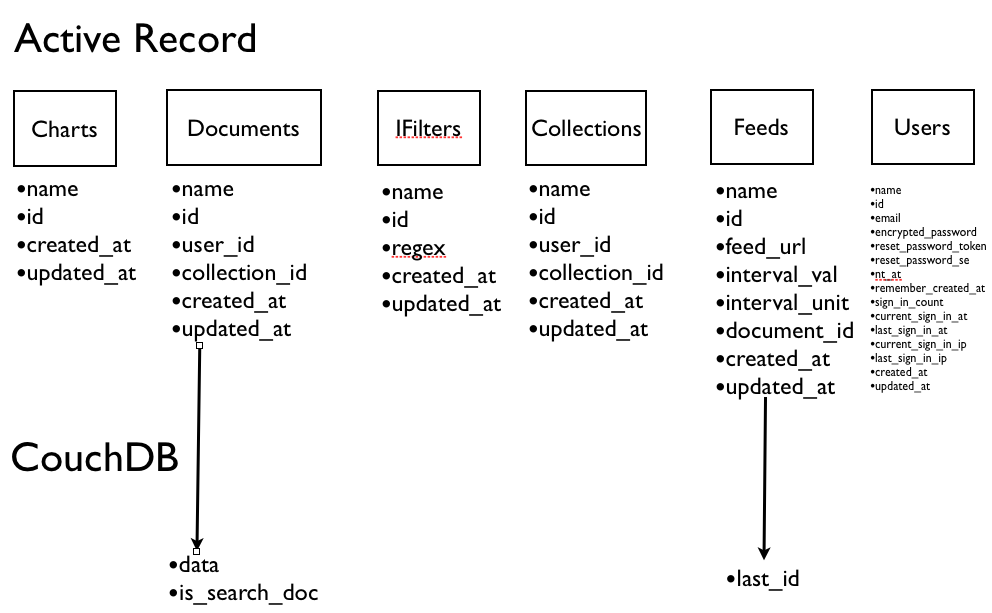
\includegraphics[width=120mm]{images/hatch_db_hybrid}
	\caption{The Hatch relational - non-relational database hybrid} 
	\label{hatch_db_hybrid}
	\end{center}
\end{figure}

The result is a relation - non-relational database hybrid. Hatch uses traditional 
relational database columns when the columns are ubiquitous, and can add columns to
a database entity (called scaffold) on the fly using CouchDB. For example, we create
a scaffold called Documents. Document always have a name, id, and collection/folder
they belong to. But, documents may have a data section, or they may not. That
data section may have infinite columns and rows of data, that would match the flat 
file they came from (like an Excel file). Or document may have any other data that
can be stored in JSON format. It is up to the Hatch interface, not database, to 
decide. And by allowing the interface to decide the structure and fields of data, Hatch
is by extension allowing the user to decide how to format data.

\pagebreak

\begin{figure}[h]
	\begin{center}
	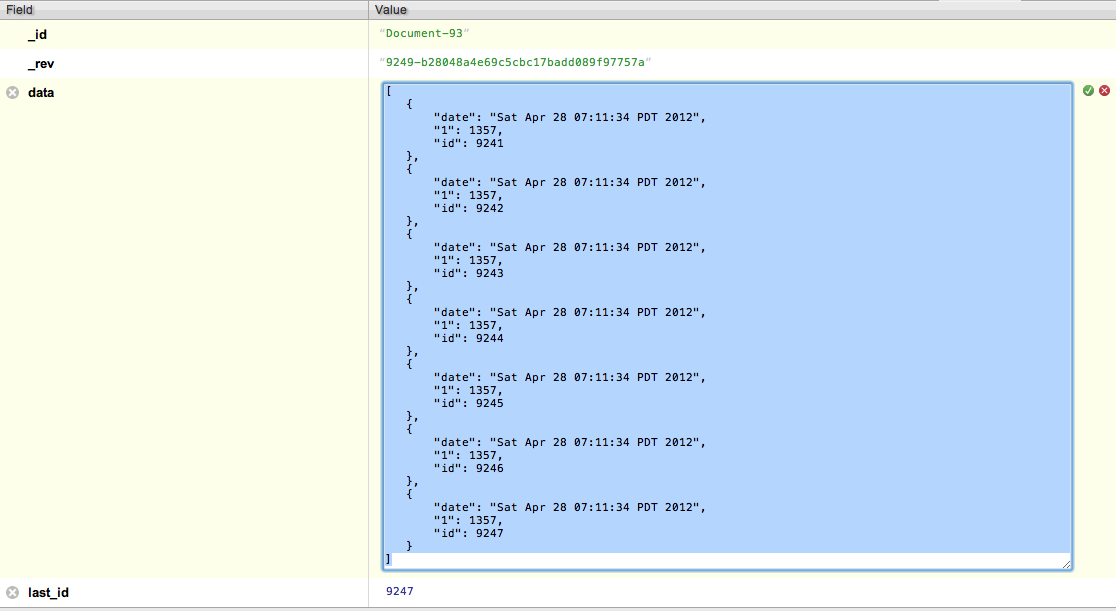
\includegraphics[width=120mm]{images/couchdb_json_ex}
	\caption{Typical representation of document data in CouchDB / JSON} 
	\label{couchdb_json_ex}
	\end{center}
\end{figure}

Most Rails applications that use CouchDB completely replace Active Record with some
library's version of it, like \textbf{couchrest's Active Model}. But if you replace
Active Record, you lose tons of support for libraries that lots of Rails developers
make, like pagination. 

Hatch gets around this by using its database hybrid, using a Ruby library called
\textbf{stuffing}. Stuffing is a link that ties Rails Active Record records with
CouchDB documents. It allows for rapid prototyping in development, and is a nice, modest
alternative to ripping out the guts of Active Record. Since the base model for 
database scaffolds are still Active Record, the huge amount of Rails Active Record based
libraries still work.



			\subsection{Documents - Requirements}
\label{sec:document_spec} 

\subsubsection{Scaffold}
The following are the requirements for Document scaffolds:
\begin{enumerate}
	\item Active Record
	\begin{enumerate}
		\item Documents shall have a \textbf{name} field.
		\item Documents shall have a \textbf{collection} field, which is an ID 
			of the parent Collection.
		\item Documents shall have a belongs\_to relationship with Collections,
			Users, and Feeds.
		\item Documents shall have a has\_many relationship with Charts.
		\item Documents shall have at least all the scaffold file generated by
			\textbf{rails generate scaffold attributes}.
	\end{enumerate}

	\item CouchDB
	\begin{enumerate}
		\item The CouchDB document will be named 'Document-<ID>', where the
			ID field is the corresponding Document ID in Active Record.
		\item All documents will have a \textbf{data} member. If empty, they
			will be an empty JSON array ( [] ).i
		\item The 'data' member is an array of hashes, and should match the
			structure that Rails Active Record has for records.
	\end{enumerate}
\end{enumerate}

\subsubsection{Scaffold - Views}
The following are requirements for Document views:
\begin{enumerate}
	\item edit - view shall be the standard rails generated view. 

	\item index - view shall start from the standard rails generated view. 
	\begin{enumerate}
		\item View shall show a Search form at the top.i
		\item If this document is a result of a search, it shall display
			a link to 'Show as Document' for search results, and then
			display the data member search results below.
		\item If a search has been submitted, then show a list of Documents
			whose names also match the search.
		\item For each Document listing displayed, display an additional link
			that allows for Document CSV download.
	\end{enumerate}

	\item edit - view shall be the standard rails generated view. 

	\item show - view shall start from the standard rails generated view. 
	Additionally:
	\begin{enumerate}
		\item View shall display the \_visualize partial.
		\item View shall display a form for data manipulation.
		\begin{enumerate}
			\item Form will have a radio button for each column that can
				manipulated.
			\item Form will have a selection list of manipulation functions.
				The only current function is \textbf{categorize}.
		\end{enumerate}
		\item View shall display all the data from the CouchDB document, as a
			html table.
		\begin{enumerate}
			\item Each cell in the data table shall be a link to Document
				Hatch Lucky Search.
		\end{enumerate}
	\end{enumerate}

\end{enumerate}


\subsubsection{Helpers}
The following are the requirements for Document Helpers:
\begin{enumerate}
	\item get\_data\_colnames(d)
	\begin{enumerate}
		\item param d - A CouchDB 'data' member of a Document. 
		\item Return - a list of all 'column names' (unique keys) from the 
			structure.
	\end{enumerate}

	\item convert\_data\_to\_native\_types(d)
	\begin{enumerate}
		\item param d - A CouchDB 'data' member of a Document. 
		\item Return - A CouchDB 'data' member of a Document, with data types
			changed from string to more explicit type, if possible.
		\item The type conversion priority is listed as follows:
		\begin{enumerate}
			\item datatime
			\item decimal/float
			\item integer
			\item string
		\end{enumerate}
	\end{enumerate}

	\item get\_data\_column(d, colname)
	\begin{enumerate}
		\item param d - A CouchDB 'data' member of a Document. 
		\item param colname - A string for the colname wanted.
		\item Return - A CouchDB 'data' member of a Document, but with only
			hashes with key == colname.
	\end{enumerate}

	\item get\_data\_map(d, colname)
	\begin{enumerate}
		\item param d - A CouchDB 'data' member of a Document. 
		\item param colname - A string for the colname wanted.
		\item Return - A CouchDB 'data' member of a Document, with unique
			values for column == colname in '1' column, and the count of
			each of the values in '2' column.
	\end{enumerate}

	\item document\_search\_data\_couch(search, lucky\_search = false)
	\begin{enumerate}
		\item param search - A string for the search value
		\item param lucky\_search - A bool value, defaults to false
		\item Return -  A CouchDB 'data' member of a Document:
		\begin{enumerate}
			\item If lucky\_search == false, a CouchDB startkey search.
			\item Else, a CouchDB key search.
		\end{enumerate}
	\end{enumerate}

\end{enumerate}

			\subsection{Collection - Requirements}
\label{sec:document_spec} 

\subsubsection{Scaffold}
The following are the requirements for Collection scaffolds:
\begin{enumerate}
	\item Collection shall start from the standard \textbf{rails generate scaffold}.
	\item Collection shall have a has\_many relationship with Documents.
	\item Collection shall have a belongs\_to relationship with Users.
	\item Collection shall have a \textbf{name} field.
\end{enumerate}

\subsubsection{Scaffold - Views}
The following are requirements for Collection views:
\begin{enumerate}
	%\item blah - view shall start from the standard rails generated view. 
	\item edit - view shall be the standard rails generated view. 

	\item index - view shall be the standard rails generated view. 
	
	\item new - view shall be the standard rails generated view. 
	
	\item show - view shall be the standard rails generated view. 

\end{enumerate}


\subsubsection{Helpers}
There are no helper requirements for Collection.

			\subsection{Home - Requirements}
\label{sec:document_spec} 

\subsubsection{Scaffold}
Home shall only have one view, and no scaffold.

\subsubsection{Scaffold - Views}
The following are requirements for Home views:
\begin{enumerate}
	\item index - a custom view.
	\begin{enumerate}
		\item View shall display a quick summary of the project.
		\item View shall list sponsors and team member names
		\item View shall link to the senior design website.
	\end{enumerate}
\end{enumerate}


\subsubsection{Helpers}
There are no helper requirements for Home.
%The following are the requirements for Home Helpers:
%\begin{enumerate}
%	\item method\_name(params)
%	\begin{enumerate}
%		\item param params - 
%		\item Return - 
%	\end{enumerate}
%\end{enumerate}

			\subsection{IFilters - Requirements}
\label{sec:document_spec} 

\subsubsection{Scaffold}
The following are the requirements for IFilters scaffolds:
\begin{enumerate}
	\item IFilters shall start from the standard \textbf{rails generate scaffold}.
	\item IFilters shall have a \textbf{name} member.
	\item IFilters shall have a \textbf{regex} member.
\end{enumerate}

\subsubsection{Scaffold - Views}
The following are requirements for IFilters views:
\begin{enumerate}
	%\item blah - view shall start from the standard rails generated view. 
	\item edit - view shall be the standard rails generated view. 

	\item index - view shall be the standard rails generated view. 
	
	\item new - view shall be the standard rails generated view. 
	
	\item show - view shall be the standard rails generated view. 

\end{enumerate}


\subsubsection{Helpers}
There are no helper requirements for IFilters.
%The following are the requirements for IFilters Helpers:
%\begin{enumerate}
%	\item method\_name(params)
%	\begin{enumerate}
%		\item param params - 
%		\item Return - 
%	\end{enumerate}
%\end{enumerate}

			\subsection{Data I/O}
\label{sec:data_io_spec} 

\subsubsection{Input}
	\begin{enumerate}
		\item The input module will allow users to import CSV native 
			formats into the metadata server’s native format.
		\begin{enumerate}
			\item \textit{Verify that the CSV inputs correctly
					into Metadata as a new Data instance.}
		\end{enumerate}
		
		\item The input module will allow creation of new input filters
			as regular expressions, to be applied to every line
			of a file, for custom file format input/importing. This
			will be implemented by the Filter scaffold (see 
			Section \ref{sec:filter}).
		\begin{enumerate}
			\item \textit{Verify that a user can specify filters
				and then apply them to correctly parse and 
				import files, per the expected behavior
				of regular expressions.}
		\end{enumerate}

		\item Once a file is inputed, the wall and system time will be
			displayed, along with the number of rows created.
		\begin{enumerate}
			\item \textit{ Verify that the wall and system time, 
					along with the number of rows, are
					displayed on input.}
		\end{enumerate}

		\item When a file is inputed, a Metadata instance will be 
			created or updated, with the 'name' field set during 
			the import.
		\begin{enumerate}
			\item \textit{ Verify that the Metadata instance is
					created with the 'name' set as the
					file name. }
		\end{enumerate}

		\item When a file is inputed, it is represented as a Data 
			instance with the 'name' field set as the name of the
			imported file.
		\begin{enumerate}
			\item \textit{ Verify that the inputed file creates 
					a new Data instance, and each row's
					name column is set to the name of the
					inputed file.}
		\end{enumerate}

		\item When a file is inputed, each column will be intepreted
			as a Rails 3 data type (see Section
			\ref{sec:data_types}). The column data type will be 
			applied to all members of all rows for the respective
			columns.
		\begin{enumerate}
			\item \textit{ Verify that a column is intepreted to
					be a support Data Type, and is inputed.}
		\end{enumerate}

		\item When a column is being considered for which Data Type
			it is, it will be attempted to be interpreted as a 
			data type in the following order, until success:
			\begin{enumerate}
				\item time
				\item date
				\item timestamp
				\item datetime
				\item boolean
				\item binary
				\item decimal
				\item float
				\item integer
				\item string
				\item text
			\end{enumerate}

		\begin{enumerate}
			\item \textit{ Verify each kind of data is intepreted
					correctly.}
		\end{enumerate}

		%\item
		%\begin{enumerate}
		%	\item \textit{ Verify }
		%\end{enumerate}
	\end{enumerate}


\subsubsection{Data Types}
\label{sec:data_types}

The supported data types are (in list of precedence):
\begin{enumerate}
	\item time
	\item date
	\item timestamp
	\item datetime
	\item boolean
	\item binary
	\item decimal
	\item float
	\item integer
	\item string
	\item text
\end{enumerate}

			\include{final_report/reportVisualization}
			\subsection{Charts - Requirements}
\label{sec:document_spec} 

\subsubsection{Scaffold}
The following are the requirements for Charts scaffolds:
\begin{enumerate}
	\item Charts shall start from the standard \textbf{rails generate scaffold}.
	\item Charts shall have a belong\_to relationship with Documents.
\end{enumerate}

\subsubsection{Scaffold - Views}
The following are requirements for Charts views:
\begin{enumerate}
	%\item blah - view shall start from the standard rails generated view. 

	\item edit - view shall be the standard rails generated view. 

	\item index - view shall be the standard rails generated view. 
	
	\item new - view shall be the standard rails generated view. 
	
	\item show - view shall be the standard rails generated view. 

\end{enumerate}


\subsubsection{Helpers}
There are no requirements for Chart helpers.

			\subsection{Visualization}
\label{sec:viz_spec}
The Visualization controller is referred to throughout documentation simply as
\textbf{Viz}. It will be Rails 3 \textbf{views} and \textbf{controllers},
without models, since it mainly inteprets data from the Metadata
\ref{sec:metadata_spec} and Data I/O \ref{sec:data_io_spec} scaffolds. There 
will be one view per controller, unless stated otherwise.

\subsubsection{Graphs - Types}

\subsubsection{Columns - Data Types}

\subsubsection{Views - Show}
	\begin{enumerate}
		\item Viz will contain one show view. 
		\begin{enumerate}
			\item \textit{Verify that there is a Show view.}
		\end{enumerate}

		\item Some other controller will pass a Data model id and 
			two column names to graph data by.
		\begin{enumerate}
			\item \textit{Verify that this view graphs the 
				correct data for the Data id and two 
				columns listed.}
		\end{enumerate}

		\item The first passed column will be \textbf{x\_data} 
			in POST, the second will by \textbf{y\_data} in 
			POST, for the respective axis.
		\begin{enumerate}
			\item \textit{Verify that the respective columns 
				graph on the correct axis.}
		\end{enumerate}

		\item Controllers may pass a graph type, but the default 
			will be a line graph type.
		\begin{enumerate}
			\item \textit{Verify that the 
				data is graphed in the correct graph types.}
		\end{enumerate}


		\item 
		\begin{enumerate}
			\item 
		\end{enumerate}

	\end{enumerate}

\subsubsection{Views - Summary}
	\begin{enumerate}
		\item Viz will contain one Summary view. This view will take in a Data model data\_id POST value, and graph every unique permutation of two columns. 
		\begin{enumerate}
			\item Verify that the Summary view graphs the correct data for data\_id.
		\end{enumerate}

		\item There will be two Summary graphs per display row.
		\begin{enumerate}
			\item Verify that there are two Summary graphs per display row.
		\end{enumerate}

		\item Summary graphs will graph 10\% or 100 points of the data, whichever is bigger.
		\begin{enumerate}
			\item Verify that Summary graphs graph 10\% or 100 points of the data.
		\end{enumerate}

		\item Summary graphs will graph any type of data as defined in Data Types (Section \ref{sec:data_types}).
		\begin{enumerate}
			\item Verify Summary graphs graph any Data Type.
		\end{enumerate}

		\item 
		\begin{enumerate}
			\item 
		\end{enumerate}

	\end{enumerate}

			\subsection{Search}
After the EcoData team addressed the issues with storing semi-structured data, the next 
big problem to address was how to efficiently search through the data. The interface 
that was desired was one much like Google's search; a simple search box, with two
buttons. The interface needs to be extremely simple yet powerful for it to be 
effective for non-technical users. 

\begin{figure}[h]
	\begin{center}
	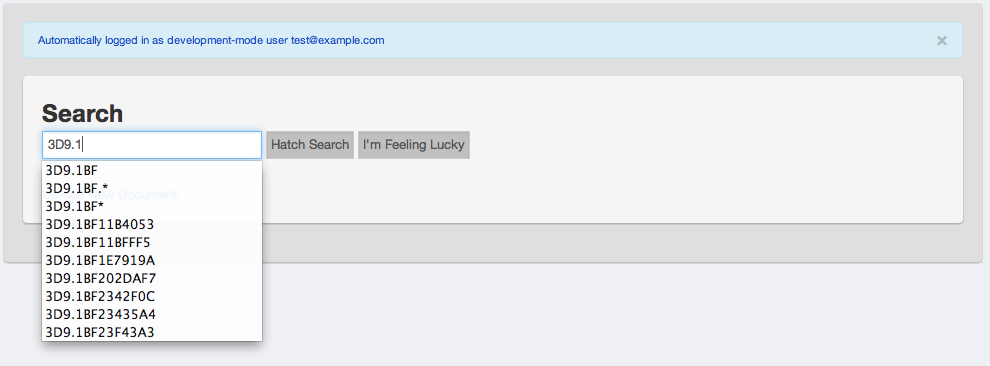
\includegraphics[width=120mm]{images/search_ss1}
	\caption{The search interface} 
	\label{search_ss1}
	\end{center}
\end{figure}

For example, when a user entered in a search like `3D9.1', it would be assumed that 
any data starting with `3D9.1' should be returned. Because Hatch assumes that
the user would want any data in the same row as the matching data, it returns
the entire row. 

For search, this could lead to a huge number of string comparisons in order to find
all values that match. This would make search impractically slow. Luckily, CouchDB allows
us to implement a practical solution to this problem.

\subsubsection{Views}
CouchDB uses precompiled queries called views. Views take developer-defined
query templates and apply them to every document that is created or updated in the 
database when the document is saved. The results are precompiled lookup tables 
(actually heaps/binary trees), which make searches fast. 

Hatch basically creates a view like the following pseudocode:
\singlespacing
\begin{lstlisting}
	for each document
		for each row
			for each column value in row
				emit(value, row)
\end{lstlisting}
\doublespacing

\texttt{emit()} is a function that tells CouchDB how to create the search B-Tree. It 
takes two arguments; the key that the tree node will take, and the value that the 
node will return if the key matches the search. Hatch says `every column value in a 
document is a key, and the return value is the data row it belongs to,' so if a search
matches a document value, the search results return the entire data row.

CouchDB makes Hatch's job easier by having internal methods for string matching. For
example, if a search for `3D9.1' is used with CouchDB startkey, CouchDB will return
any string starting with `3D9.1'. Hatch doesn't have to invent a query language to 
tell the database lots of parameters for matching values, which means users do not
need to learn a new query language either.

\begin{figure}[h]
	\begin{center}
	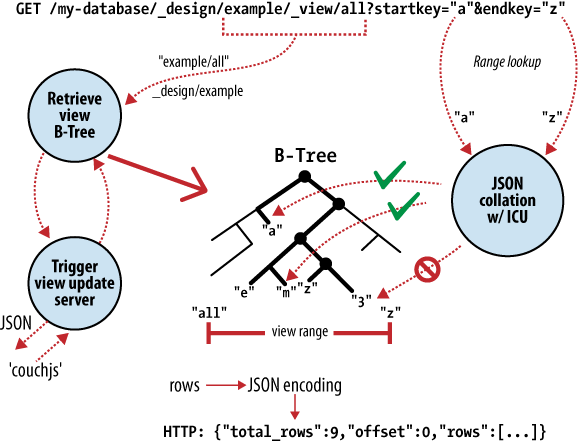
\includegraphics[width=120mm]{images/couchdb_b_tree}
	\caption{CoucbDB search through its internal binary tree.} 
	\label{couchdb_b_tree}
	\end{center}
\end{figure}

The other advantage to CouchDB is that it stores values in the B-Tree structure. For
string data types, this means that the database searches only within the `3D9.1' string range
in the tree. When the search sees a child node starting with `3D9.0', it instead picks
the child node staring with `3D9.1', and the entire `3D9.0' group is never searched 
through, which makes searches complete in a short time frame. 

			%\include{SSRS/SearchRequirements}


\begin{comment}
\part{Systems and Software Requirements Specification (SSRS) \\ for \\ Hatch}

\chapter{Overall Description}

%------------------------------------------------

	\section{Product Perspective}
				Gus is an independent software system, as it does not directly
		integrate with a larger system. However, GUS does draw data from
		external sources, such as personal information databases, and
		needs to be integrated with a web server in order to be readily
		accessible.
	\section{Product Functions}
				\begin{enumerate}
		\item Simplifying tasks to leaders of groups, such as:
			\begin{enumerate}
				\item Sending notifications to group members, prospective
					members, former members, and interested community
					members (email)
				\item Sending information (files) to group members via
					email or download link
				\item Managing a group-wide calendar of events
				\begin{enumerate}
					\item track volunteers, attendees, and contributors
					\item suggest potentially beneficial services other
						groups could provide related to the event
					\item provide a calendar of events that includes events
						from other groups that members would want to attend
						(like marching band if half of LCM are in the
						marching	band.)
					\item keeping track of who is responsible for bringing
						/ doing what at an event
				\end{enumerate}
				\item Automatically generating:
				\begin{enumerate}
					\item Contact information (contact sheets, phone
						directories)
					\item Website with updated contact, group, event, and
						customized information
					\item Organization charts
					\item Graphical relationships between groups
					\item Fees, dues, and expenses notifications
					\item Event reminders
				\end{enumerate}
			\end{enumerate}
			\item Consolidating information for members, former members,
				potential members (and parents) of groups:
			\begin{enumerate}
				\item Common location of group information
				\item Searching existing groups
				\item Tying together existing groups (even suggesting
					similar groups)
				\item Personalized emails regarding changes/updates
				\item Outstanding expenses or reimbursements
				\item Reliable (i.e., automatically updated):
				\begin{enumerate}
					\item Group contact information
					\item Group event information
				\end{enumerate}
				\item Transcript of verified group activity (for use with
					service-learning classes, and proof of volunteerism
					for potential employers)
				\item Supplementing Vandal Friday with emails to
					prospective high school Seniors
			\end{enumerate}
			\item Getting member input though: forums, project managers,
				surveys, and polls
			\item Payment processing and sponsorship collection
			\item 4. Recruitment and advertising for groups, volunteer
				/ paid opportunities, services provided, possibly a
				bartering tool
		\end{enumerate}
	\section{User Characteristics}
				Gus should be easy for any user to understand with a brief
		explanation and intuitive enough for an uninitiated user to
		figure out by looking through the options. Basic computer use
		skills and a simple conceptual explanation should be enough for
		every day usage.
	\section{Constraints}
				GUS must meet privacy policies as they apply to both the
		University of Idaho and social networking sites.  GUS must be
		able to interface with outside database servers (such as the
		Center for Volunteerism's database, UI's career seeker site,
		common social networks, and parent groups of university groups).
		Member's activities and group's activities must be audited for
		accuracy and safety.  The languages used to program GUS will be
		primarily, HTML, CSS, and PHP for the user interface, C++ for
		the interface between the user interface (which will implement
		security and complex business rules), and the database, and
		SQL for the database.  The networking protocols will be TCP/IP
		and Open MP / MPI will be used to enhance parallel operation.
		The system will have personal information for over 5,000
		students, so confidentiality is of the utmost importance.
	\section{Assumptions and Dependencies}
				The software system should run like a web-app and need not be
		downloaded by users.  It is assumed that users will be running
		Internet Explorer, Fire Fox, or another popular web browser.
		The server for the system is expected to run a UNIX operating
		system.
	\section{System Level (Non-Functional) Requirements}
		\subsection{Site dependencies}
			GUS will require a server that can support 1,000 concurrent
			users.  The database must store the information, interests,
			and activities of approximately 5,000 external users, 5,000
			students and 200 groups.
		\subsection{Safety, security and privacy requirements}
			GUS contains the personal information of over 5,000 users
			security should be integrated into every facet of this
			program.  The privacy criteria for this system must reflect
			privacy policies that apply to the University of Idaho, and
			the security criteria for this system must reflect the need
			to secure over 5,000 users from identity theft and potential
			defamation of character.
		\subsection{Performance requirements}
		\begin{enumerate}
			\item The number of simultaneous users to be supported are: 1,000.
			\item Supported information ranges from text to files to streaming video.
			\item 95\% of the transactions shall be processed in less than half a second.
		\end{enumerate}
		\subsection{System and software quality}
			Gus must perform all required functions, behave consistently
			and correctly, be easily corrected, running between 5:30 am
			all day to 1:30 am be easily adaptable, test-driven, and easy
			to use.
		\subsection{Packaging and delivery requirements}
			The executable system and all associated documentation (i.e.,
			SSRS, SDD, code listing, test plan (data and results), and
			user manual) will be delivered to the customer via Internet
			download. The final, edited version of the above documents
			will accompany the final, accepted version of the executable system.
		\subsection{Personnel-related requirements}
			The system under development will require a graduate student
			system-level administrator to maintain the system.
		\subsection{Training-related requirements}
			No training materials or expectations are tied to this
			project other than the limited help screens built into the
			software and the accompanying user manual.
		\subsection{Logistics-related requirements}
			A server will be required to maintain the software system.
			The user will be required to have an Internet connection.
		\subsection{Precedence and criticality of requirements}
			\begin{enumerate}
				\item Maintaining confidentiality and privacy of PII
				\item This system must be reliable enough for users to not
					give up on it
				\item All other features are less important than the first
					two and equally important
			\end{enumerate}
\chapter{Specific Requirements}
	\section{External Interface Requirements}
		\subsection{Hardware Interfaces}
			The system will require a server and secure networking
			abilities.
		\subsection{Software Interfaces}
			The system will require an interface to interact with
			emailing systems, databases, and authentication servers.
		\subsection{User Interfaces}
			The system will require user interfaces for non-university
			users (prospective students, community members, alumni,
			parent groups, etc.), students, officers, and staff/faculty.
		\subsection{Other Communication Interfaces}
			 GUS will interface with the university career seeking site
			 and social networking sites.
			 \pagebreak
			 \begin{landscape}
		\begin{table} \caption{Hardware Interfaces}
		\begin{tabular}{|p{1.75cm}|p{4cm}|p{5.25cm}|p{2.5cm}|p{3cm}|p{1.75cm}|} \hline
								%% Titles
			 \textbf{Name}
			 & \textbf{Source/Destination}
			 & \textbf{Description}
			 & \textbf{Type/range}
			 & \textbf{Dependencies}
			 & \textbf{Formats}
			 \\\hline
			 %% row 2
			 HTTP Server
			 & Dedicated Server or VPS / Client
			 & This device is responsible for serving HTML content (and
			   other content) to clients. Preferably Apache2.
			 & All
			 & Requires a server-capable machine
			 & N/A
			 \\\hline
			 %% row 3
			 VPS or Dedicated Server
			 & NA
			 & A VPS or a Dedicated Server, preferably running a
			   preconfigured Linux distribution such as Fedora or Ubuntu.
			 & All
			 & Electricity, high-speed Internet connection
			 & N/A
			 \\\hline

		\end{tabular} \end{table}
		\begin{table} \caption{Software Interfaces}
		\begin{tabular}{|p{1.75cm}|p{4cm}|p{5.25cm}|p{2.5cm}|p{3cm}|p{1.75cm}|}
		\hline
								%% Titles
			 \textbf{Name}
			 & \textbf{Source/Destination}
			 & \textbf{Description}
			 & \textbf{Type/range}
			 & \textbf{Dependencies}
			 & \textbf{Formats}
			 \\\hline
			 %% row 2
			 SQL Server
			 & Dedicated Server or VPS / Client
			 & Works in conjunction with HTTP server to provide data.
			 & All
			 & Requires a server-capable machine
			 & N/A
			 \\\hline
			 %% row 3
			 PHP5
			 & HTTP Server / Client
			 & Provides computational power so tasks that serve HTML
			   content via apache can be completed.
			 & Requires a server capable of running PHP5.
			 & Electricity, high-speed Internet connection
			 & N/A
			 \\\hline
			 \end{tabular}
			 \end{table}
		\begin{table} \caption{User Interfaces}
		\begin{tabular}{|p{1.75cm}|p{4cm}|p{5.25cm}|p{2.5cm}|p{3cm}|p{1.75cm}|}
		\hline
								%% Titles
			 \textbf{Name}
			 & \textbf{Source/Destination}
			 & \textbf{Description}
			 & \textbf{Type/range}
			 & \textbf{Dependencies}
			 & \textbf{Formats}
			 \\\hline
			 %% row 2
			 Website
			 & HTTP Server/Client
			 & Allows user to interact with the service
			 & All
			 & HTTP Server
			 & Web
			 \\\hline
			 %% row 3
			 Cell phone
			 & Cellphone
			 & Receive text-messages
			 & All
			 & HTTP Server
			 & Text
			 \\\hline
			 \end{tabular}
			 \end{table}
			\begin{table} \caption{Other Communication Interfaces}
			\begin{tabular}{|p{1.75cm}|p{4cm}|p{5.25cm}|p{2.5cm}|p{3cm}|p{1.75cm}|}
			\hline
								%% Titles
			 \textbf{Name}
			 & \textbf{Source/Destination}
			 & \textbf{Description}
			 & \textbf{Type/range}
			 & \textbf{Dependencies}
			 & \textbf{Formats}
			 \\\hline
			 %% row 2

			 &
			 &
			 &
			 &
			 &
			 \\\hline
			 \end{tabular}
			 \end{table}
			 \end{landscape}
	\pagebreak

%------------------------------------------------

	\section{System Features}
		\subsection{Use Case Diagrams}
		This is an example Use Case.

\end{comment}
%----------------------------------------------- back matter of the document
%\appendix                                      % following chapters are appendixes
\end{document}
